% !TEX TS-program = pdflatex
% !TEX encoding = UTF-8 Unicode

\documentclass[10pt,twocolumn]{article}

\usepackage{graphicx,listings,fixltx2e,lambda,array,times,fullpage}
\usepackage[usenames,dvipsnames]{xcolor}
\usepackage{color}

\definecolor{lightgray}{rgb}{0.92,0.92,0.92}

\lstset{ 
  language=Python,                % the language of the code
  linewidth=220pt, 
  xleftmargin=8pt,
  basicstyle=\footnotesize\ttfamily, % Standardschrift
  numbers=none,                   % where to put the line-numbers
  numberstyle=\footnotesize,          % the size of the fonts that are used for the line-numbers
  stepnumber=1,                   % the step between two line-numbers. If it's 1, each line 
                                  % will be numbered
  numbersep=5pt,                  % how far the line-numbers are from the code
  showspaces=false,               % show spaces adding particular underscores
  showstringspaces=false,         % underline spaces within strings
  showtabs=false,                 % show tabs within strings adding particular underscores
  frame=single,                   % adds a frame around the code
  tabsize=2,                      % sets default tabsize to 2 spaces
  captionpos=b,                   % sets the caption-position to bottom
  breaklines=true,                % sets automatic line breaking
  breakatwhitespace=false,        % sets if automatic breaks should only happen at whitespace
  title=\lstname,                   % show the filename of files included with \lstinputlisting;
                                  % also try caption instead of title
  numberstyle=\tiny\color{gray},        % line number style
  keywordstyle=\color{blue},          % keyword style
  commentstyle=\color{dkgreen},       % comment style
  backgroundcolor=\color{lightgray}, 
  belowskip=-10pt, 
  aboveskip=6pt, 
}


\begin{document}

\title{Parakeet: A Just-In-Time Parallel Accelerator for Python}
\author{
Alex Rubinsteyn \ \ \ \ Eric Hielscher \ \ \ \ Nathaniel Weinman \ \ \ \
Dennis Shasha \\
{\it Computer Science Department, New York University, New York, NY, 10003} \\
\small{\tt \{alexr,hielscher,nsw233,shasha\} @ cs.nyu.edu}
}
\date{}

% define some useful commands to use in language specification 
\newcommand{\MAP}{\impfnt{map}}
\newcommand{\REDUCE}{\impfnt{reduce}}
\newcommand{\SCAN}{\impfnt{scan}}
\newcommand{\ALLPAIRS}{\impfnt{allpairs}}
\newcommand{\concat}{\ensuremath{+\!\!\!\!+\,}}

\setlength\fboxsep{8pt}
\setlength\fboxrule{0.5pt}

\maketitle

\begin{abstract}
High level productivity languages such as Python or Matlab enable the use of computational resources by non-expert programmers.  However, these languages sacrifice program speed for ease of use, with this trade-off especially stark for modern parallel processors such as multicore CPUs and manycore GPUs.

In this paper, we discuss Parakeet, a library which provides a just-in-time (JIT) parallel accelerator for Python.  Parakeet bridges the gap between the usability of Python and the speed of code written in efficiency languages such as C++ or CUDA.  Parakeet accelerates data-parallel sections of Python that use the standard NumPy scientific computing library.  Parakeet automatically JIT compiles efficient versions of Python functions and manages their execution on both GPUs and multicore CPUs.  We assess Parakeet on a pair of benchmarks and exhibit significant speedups.  We use these current results as a basis for discussing our plans to augment the Parakeet feature set.
\end{abstract}

\section{Introduction}
\label{Intro}
Computers are indispensable tools to professionals in a wide range of fields, from the natural sciences to the financial industry.  Often, users in these fields either (1) aren't expert programmers; or (2) don't have time to spend tuning their software for performance.  Thus, these users typically prefer to use productivity languages such as Python or Matlab rather than efficiency languages such as C++.  Productivity languages facilitate non-expert programmers by trading off program speed for ease of use \cite{Pre03}.

A common problem, however, is that the performance tradeoff is often very stark -- code written in Python or Matlab~\cite{Moler80} often has much worse performance than code written in C++ or Fortran.  This problem is getting worse, as modern processors (multicore CPUs as well as GPUs) are all parallel, and current implementations of productivity languages are poorly suited for parallelism.  Thus a common workflow involves prototyping of algorithms in a productivity language, followed by porting the performance-critical sections to a language with better performance.  This second step can be time-consuming, error-prone, and it diverts energy from the real focus of these users' work.

In this paper, we present Parakeet, a library that provides a JIT parallel accelerator for NumPy, the commonly-used scientific computing library for Python~\cite{Oliphant07}. Parakeet accelerates performance-critical sections of numerical Python programs to be competitive with efficiency language code, obviating the need for the above-mentioned ``prototype, port'' cycle.

The Parakeet library intercepts programmer-marked functions and uses high-level operations on NumPy arrays (e.g.~mapping a function over the array's elements) as sources of parallelism. These functions are just-in-time compiled to either x86 machine code using LLVM~\cite{Latt02}, or GPU programs that can be executed on NVIDIA GPUs via the CUDA framework~\cite{NvidCU}. These native versions of the functions are then automatically executed on the appropriate hardware. Parakeet allows complete interoperability with all of the standard Python tools and libraries.

Parakeet currently supports JIT compilation to parallel GPU programs and single-threaded CPU programs.  While Parakeet is a work in progress, our current results clearly demonstrate its promise.  In the near future, Parakeet's CPU support will be extended to make better use of modern multicore CPUs.  This includes adding support for splitting computations across CPUs and GPUs simultaneously -- keeping all processors in a system busy at once -- and on-the-fly tuning of resource usage.

\section{Overview}
\label{overview}

Parakeet is an accelerator library for numerical Python algorithms written using the NumPy array extensions~\cite{Oliphant07}. Parakeet does not replace the standard Python runtime but rather selectively augments it. To run a function within Parakeet a user must wrap it with the decorator \lstinline{@PAR}. For example, consider the following NumPy code for computing the entropy of a discrete probability distribution: 
\begin{lstlisting}
  @PAR
  def entropy(p):
    return -numpy.sum(p * numpy.log2(p))
\end{lstlisting}
If the decorator \lstinline{@PAR} were removed, then \lstinline{entropy} would run as ordinary Python code. Since NumPy's \lstinline{log2} and array multiplication operators are statically compiled they always allocate result arrays (even when they are immediately consumed). In contrast, Parakeet specializes the function \lstinline{entropy} for any distinct input type, optimizes the body into a singled fused reduction (avoiding unnecessary allocation) and executes it as parallel native code.

Parakeet is not meant as a general-purpose accelerator for all Python programs.  Rather, it is designed to execute array-oriented numerical algorithms such as those found in machine learning, financial computing, and scientific simulation. In particular, the sections of code that Parakeet accelerates must obey the following constraints:

\begin{itemize}
 \item Due to the difficulty of implementing efficient non-uniform data structures on the GPU, we require all values within Parakeet to be either scalars or NumPy arrays. No dictionaries, sets, or user-defined objects are allowed. 
 \item To compile Python into native code we must assign types to each expression. We are still able to retain some of Python's polymorphism by specializing different typed versions of a function for each distinct set of argument types. However, expressions whose types depend on dynamic values are disallowed (e.g.~\lstinline{43 if bool_val else "sausage"}).
 \item Only functions which don't modify global state or perform I/O can be executed in parallel. Local mutabable variables are  always allowed.
\end{itemize}

These restrictions would be onerous if applied to an entire program, but it's important to remember that Parakeet only sees the computational core of an algorithm. All other code is executed as usual by the Python interpreter. Furthermore, the style of programming required for Parakeet closely matches the idiomatic conventions of array programming. In practice, if an algorithm makes heavy use of NumPy operators for its computations then it will run under Parakeet with only minor modifications. 


Though Parakeet supports the use of loops, it does not attempt to parallelize them in any way. Parallelism is instead achieved by relaxing the iteration order of the following higher-order array operators:

\begin{itemize}
\item $\MAP(\textit{f}, \; \textit{X}_1,  ... ,  \textit{X}_n, \; \textit{fixed}\textrm{=[]}, \; \textit{axis}\textrm{=None})$ \\
  Apply the function \textit{f} to each element of the array arguments. By default, \textit{f} is passed each scalar element of the array arguments. \\
  The \textit{axis} keyword can be used to specify a different iteration pattern (such as applying \textit{f} to all columns). 
  The \textit{fixed} keyword is a list of values which precede the array elements as arguments to \textit{f} (simulating partial function application). 
       
\item $\ALLPAIRS(\textit{f}, \; \textit{X}_1,  \; \textit{X}_2, \; \textit{fixed}\textrm{=[]}, \; \textit{axis}\textrm{=} 0)$ \\
  Apply the function \textit{f} to each pair of elements from the arrays \textit{X}$_1$ and \textit{X}$_2$.   
\item $\REDUCE(\textit{f}, \; \textit{X}_1,  ... ,  \textit{X}_n, \; \textit{fixed}\textrm{=[]}, \; \textit{axis}\textrm{=None}, \; \textit{init}\textrm{=None})$ \\
  Combine all the elements of the array arguments using the $n+1$-ary commutative operator $f$. Examples of reductions are the NumPy functions \lstinline{sum} and \lstinline{product}. 
\item $\SCAN(\textit{f}, \; \textit{X}_1,  ... ,  \textit{X}_n, \; \textit{fixed}\textrm{=[]}, \; \textit{axis}\textrm{=None}, \;  \textit{init}\textrm{=None})$ \\
  Combine all the elements of the array arguments and return an array containing all cumulative intermediate values of the combination. 
  Examples of scans are the NumPy functions \lstinline{cumsum} and \lstinline{cumprod}. 
\end{itemize}

For each occurrence of a data parallel operator in a user's program Parakeet may choose, based on heuristics discussed later, to synthesize parallel code which performs the same computation. It is not always necessary, however, to explicitly use one of these operators in order to achieve parallelization. 
Parakeet implements NumPy's array broadcasting semantics by implicitly inserting calls to $\MAP$ into a user's code. Furthermore, Parakeet reimplements a subset of the NumPy library functions (\lstinline{sum}, \lstinline{argmax}, etc...) in order to expose opportunities for parallelism.



\section{Parakeet Runtime and Internals}
To convey a more concrete understanding of how Parakeet works internally we utilize two example functions taken from our K-Means clustering benchmark. The function \lstinline{minidx} takes as input a matrix \lstinline{C} and a vector \lstinline{x} and then computes the index of the row in \lstinline{C} whose distance from \lstinline{x} is smallest.

\begin{lstlisting}[language=Python,frame=single, label=MinIdx]
def sqr_dist(x,y):
  return sum((x-y) * (x-y))

@PAR
def minidx(C,x):
  sqr_dists = map(sqr_dist,C,fixed=[x])
  return argmin(sqr_dists)
\end{lstlisting}

When the Python interpreter starts running it calls the decorator \lstinline{PAR} with \lstinline{minidx} as its argument. Parakeet's front-end 
translates the syntax tree of \lstinline{minidx} into Parakeet's untyped internal language representation, which is then converted to Static Single Assignment form \cite{Cytr91}. 


\subsection{Type Specialization}
Whenever \lstinline{minidx} is called from within Python, Parakeet intercepts its arguments and uses their types to synthesize a typed version of the function's body. For example, if the types of the arguments were \lstinline{array2(float), array1(float)} then a specialized version of \lstinline{minidx} would be synthesized just for those types. Furthermore, the specialization process would recursively trigger the specialization of \lstinline{sqr_dist} for argument types \lstinline{array1(float), array1(float)}. 

In Parakeet's typed representation, every function must have unambiguous input and output types. To eliminate polymorphism Parakeets inserts casts and $\MAP$ operators where necessary. When \lstinline{sqr_dist} is specialization for vector arguments, its math operators are rewritten into one-dimensional $\MAP$s of those same operators. 

The actual process of type specialization is implemented by interleaving an abstract interpreter which propagates input types to infer local types and a rewrite engine which inserts coercions where necessary. 


Parakeet performs optimizations both before and after type specialization. We subject the untyped representation to inlining, common subexpression elimination, constant propagation and dead code elimination. This step occurs once for each function, upon its first interception by Parakeet. It is preferable to eliminate as much code as possible at this early stage since an untyped function body serves as a template for a potentially large number of future specializations. The only optimizations we do not perform on the untyped representation are array fusion rewrites, since these rely on type annotations to ensure correctness.

Specialization transform user programs from the untyped intermediate language into its typed variety. The purpose of this transformation is to eliminate polymorphism, to make manifest all implicit behavior (such as coercion and scalar promotion), and to assign simple unboxed types to all data used within a function body. 

\subsection{Optimization}
In addition to standard compiler optimizations (such as constant folding, function inlining, and common sub-expression elimination), we employ fusion rules~\cite{Jones01} to combine array operators. Fusion enables us to minimize kernel launches, boost the computational density of generated kernels, and avoid the generation of unnecessary array temporaries.

Further standard optimizations are performed at this stage, the most impactful of which is \emph{array operator fusion}, wherein array operations are combined according to rewriting rules. 

\subsection{Execution}

Execution of the optimized typed IL is initiated by Parakeet's interpreter, which is then responsible for deciding which operations to JIT compile to native code for the CPU or GPU. When the interpreter encounters an array operator it employs a simple cost-based heuristic (which considers nested array operators, data sizes, and memory transfer costs) to decide where to execute it 

If an array operator's computation is deemed a good candidate for native hardware execution, Parakeet flattens all nested array computations within that operator into sequential loops.  This payload is then inlined into a program skeleton that implements that operator.  For example, in the case of a \textbf{map} operation, Parakeet provides skeletal algorithms that implement the pattern of applying the same function to each element of an array on the CPU as well as on the GPU.  The flattened payload function argument is inlined into this skeleton, and a complete program is synthesized and JIT compiled.

To execute the native code, Parakeet first copies any of its inputs that aren't already present in the memory of the target hardware to their necessary place.  Parakeet manually manages the memory of the system, for example treating the GPU's memory as a cache of data whose canonical values are the CPU's RAM. The program is then executed, with memory reclaimed via garbage collection.

\begin{figure*}[t!bh]
\begin{center}
\leavevmode
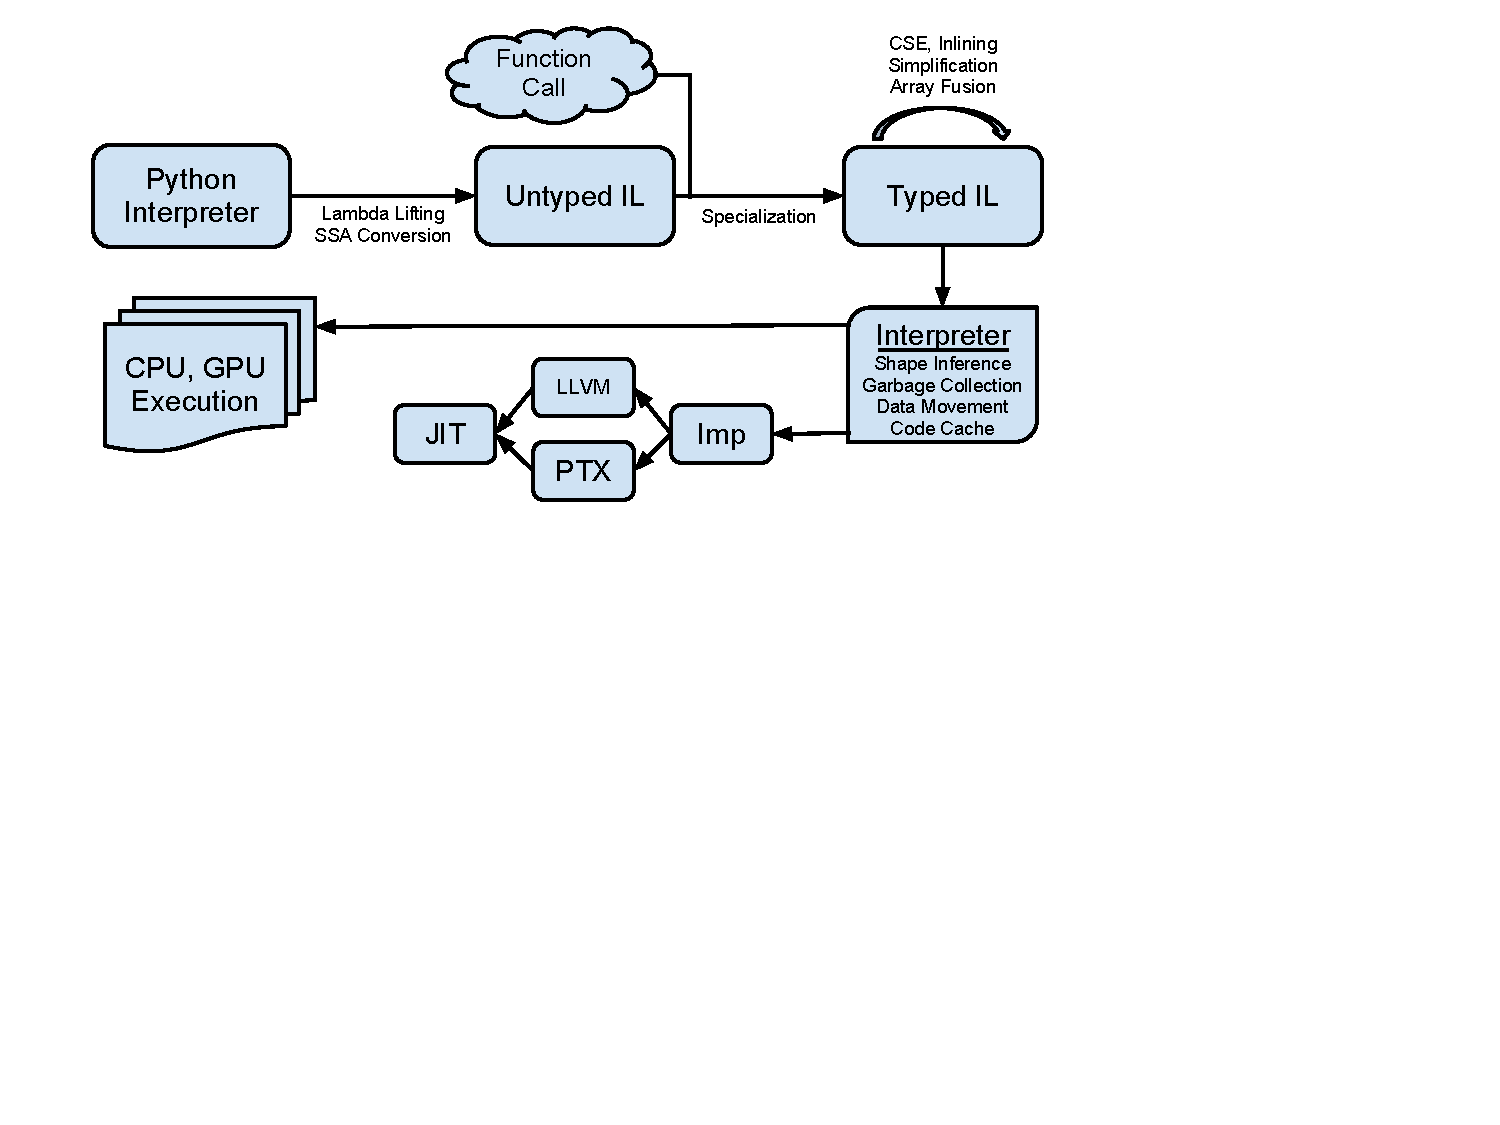
\includegraphics[scale=0.6, trim=0pt 310pt 140pt 80pt]{ParakeetNumPyOverview.pdf}
\end{center}
\caption{Parakeet Pipeline}
\label{fig:overview}
\end{figure*}

\section{The Parakeet Runtime}
\label{runtime}

Once a function has been type specialized and fully optimized, it is handed off to the Parakeet runtime for intelligent execution. The heart of the runtime is a heavy-weight interpreter whose primary responsibility is to initiate GPU kernel synthesis and execution. The interpreter uses program analyses and performance heuristics in order to dynamically make decisions such as: 
\begin{enumerate}
\item what portion of a user's program ought to run on the GPU 
\item which level of nested parallelism ought to expressed as a GPU kernel
\item in which GPU memory space should a particular array reside 
\item when should data be moved onto or off the GPU
\end{enumerate} 

Accurate prediction of array shapes is necessary both for the allocation of intermediate values on the GPU as well as for the above cost model determining placement of computations. We employ a simple abstract interpreter which propagates shape information through a function using the obvious shape semantics for each operator. For example, a $\REDUCE$ operation collapses the outermost dimension of its argument whereas a $\MAP$ preserves a shape's outermost dimension.

When the Parakeet interpreter encounters an array operator, it uses a simple cost model to decide what is the best place to execute the operator.  For a $\MAP$ operation, for example, we multiply the estimated cost of performing the sequentialized version of the mapped function by the number of input elements. In addition, we estimated the time needed to transfer data to and from the GPU as a function of data size and add this cost to the total if the data is not already present in the respective processor's memory.

In the case of nested array operators -- e.g.~a $\MAP$ whose payload function is itself a $\REDUCE$ the interpreter needs to choose which operator, if any, will form the parallelization point for a GPU kernel while sequentializing all nested operators within that kernel.  The possible choices include:

\begin{enumerate}
\item Running the \textbf{map} as a GPU kernel, with an embedded sequential \texttt{for} loop that implements the \textbf{reduce}.
\item Running the \textbf{map} as a \texttt{for} loop in the Parakeet interpreter, with each iteration of the loop calling a GPU kernel that implements the \textbf{reduce}.
\item Running everything in the Parakeet interpreter as two nested \texttt{for} loops.
\end{enumerate}



\section{GPU Back End}
Several systems similar to Parakeet \cite{Cata11,Chaf11} generate GPU programs by emitting CUDA code which is then compiled by NVIDIA's CUDA nvcc toolchain. Parakeet on the other hand, targets PTX, which is NVIDIA's GPU pseudoassembly language. Parakeet's PTX code is dynamically compiled by the NVIDIA graphics driver before being executed.  We prefer compiling PTX instead of CUDA since the compile times are dramatically shorter. 

Arrays are moved to the GPU whenever they are used as the argument to some GPU computation. The specific GPU memory space into which an array is loaded depends on both the other data already on the GPU and the individual characteristics of the computation in which that array is being used.
Unlike some systems similar to Parakeet \cite{Chaf11}, we do not by default preallocate the entirety of the GPU's memory. 

\section{Evaluation}
\label{Evaluation}

We evaluate Parakeet on two benchmarks: Black-Scholes option pricing, and K-Means Clustering.  We compare Parakeet against hand-tuned CPU and GPU implementations.  Due to space constraints, and since at the time of writing our CPU backend only supports single-threaded execution, we only present GPU results for Parakeet.  For Black-Scholes, the CPU reference implementation is taken from the PARSEC \cite{Bien08} benchmark suite, and the GPU implementation is taken from the CUDA SDK \cite{NvidSD}.  For K-Means Clustering both the CPU and GPU reference versions come from the Rodinia benchmark suite~\cite{Che09}.

We ran all of our benchmarks on a machine running 64-bit Linux with an Intel Core i7 3.2GHz 960 4-core CPU  and 16GB of RAM.  The GPU used in our system was an NVIDIA Tesla C1060 with 240 vector lanes, a clock speed of 1.296 GHz, and 4GB of memory.

\subsection{Black-Scholes}
\label{results-bs}

Black-Scholes option pricing \cite{Blac73} is a standard algorithm used for data parallel benchmarking.  We compare Parakeet against the multithreaded OpenMP CPU implementation from the PARSEC \cite{Bien08} suite with both 1 and 8 threads and the GPU version in the CUDA SDK \cite{NvidSD}.  We modified the benchmarks to all use the input data from the PARSEC implementation so as to have a direct comparison of the computation alone.  We also modified the CUDA version to calculate only one of the call or put price per option so as to match the behavior in PARSEC.

\begin{figure}[h!]
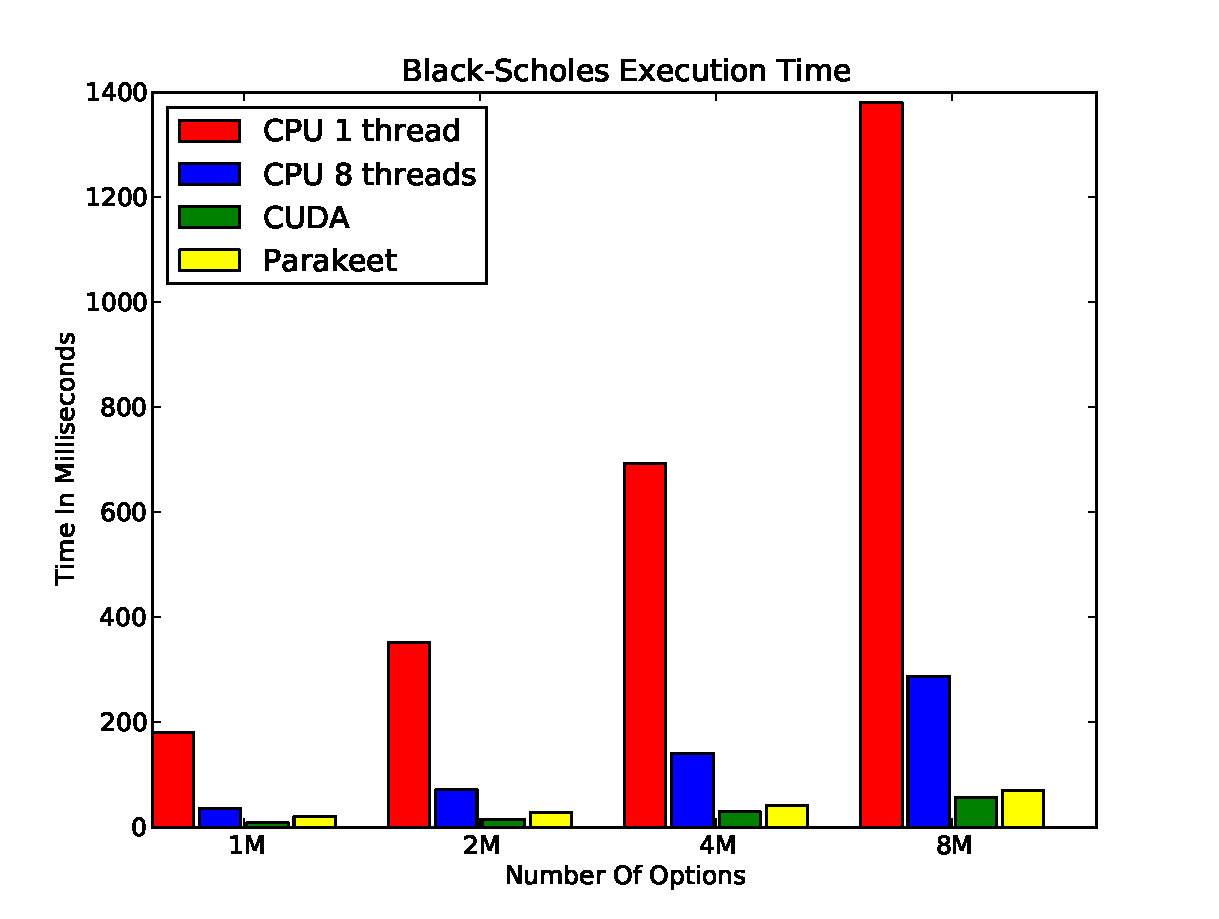
\includegraphics[scale=0.4]{BSWCPU.pdf}
\caption{Black Scholes Total Times}
\label{BSCPU}
\end{figure}

In Figure \ref{BSCPU}, we see the total run times of the various versions. These times include the time it takes to transfer data to and from the GPU in the GPU benchmarks.  As expected, Black Scholes performs very well on the GPU as compared with the CPU.  We see that Parakeet performs very similarly to the hand-written CUDA version, with overheads decreasing as a percentage of the runtime as the data sizes grow since most of them are fixed costs related to dynamic compilation.

\subsection{K-Means Clustering}
\label{results-k-means}

\begin{figure}
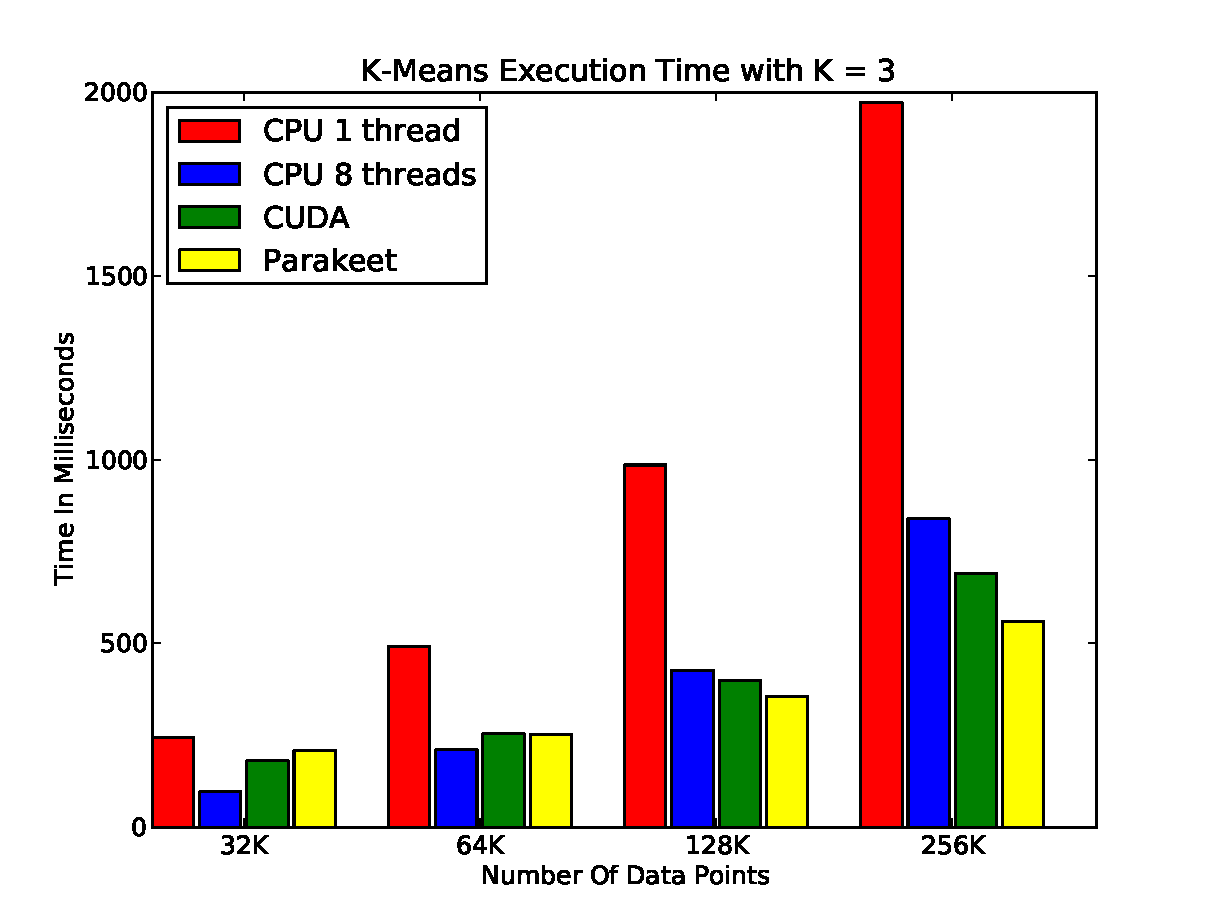
\includegraphics[scale=0.4]{KMCPUK3.pdf}
\caption{K-Means Total Times with 30 Features, K = 3}
\label{KMCPU3}
\end{figure}

We also tested Parakeet on K-Means clustering, a commonly used unsupervised learning algorithm.  We chose K-Means since it includes both loops and nested array operators, and thus illustrates Parakeet's support for both.

In Figure \ref{KMCPU3}, we see the total run times of K-Means for the CPU and GPU versions with K = 3 clusters and 30 features on varying numbers of data points.  Here, the distinction between the GPU and the CPU is far less stark.  In fact, for up to 64K data points the 8-thread CPU version outperforms the GPU.  Further, we see that on all but the smallest input size, Parakeet actually performs better than both the CPU and GPU versions.

The reason Parakeet is able to perform so well with respect to the CUDA version is due to the difference in how the two versions execute the code that computes the new average centroid for the new clusters in each iteration.  The CUDA version brings the GPU-computed assignment vectors back to the CPU in order to perform this reduction, as it involves many unaligned memory accesses and so has the potential to perform poorly on the GPU.  Parakeet executes code to perform this function on the GPU instead, prefering to avoid the data transfer penalty.  For such a small number of clusters, the Parakeet method ends up performing far better.  However, for larger numbers of clusters (roughly 30 and above), the fixed overhead of launching an individual kernel to average each cluster's points overwhelms the performance advantage the GPU gives and Parakeet ends up performing worse than the CUDA version.  We are currently implementing ways of using dynamic information in order to use the GPU only when it would actually be advantageous, in which case Parakeet should perform well for all numbers of clusters.

\begin{figure}
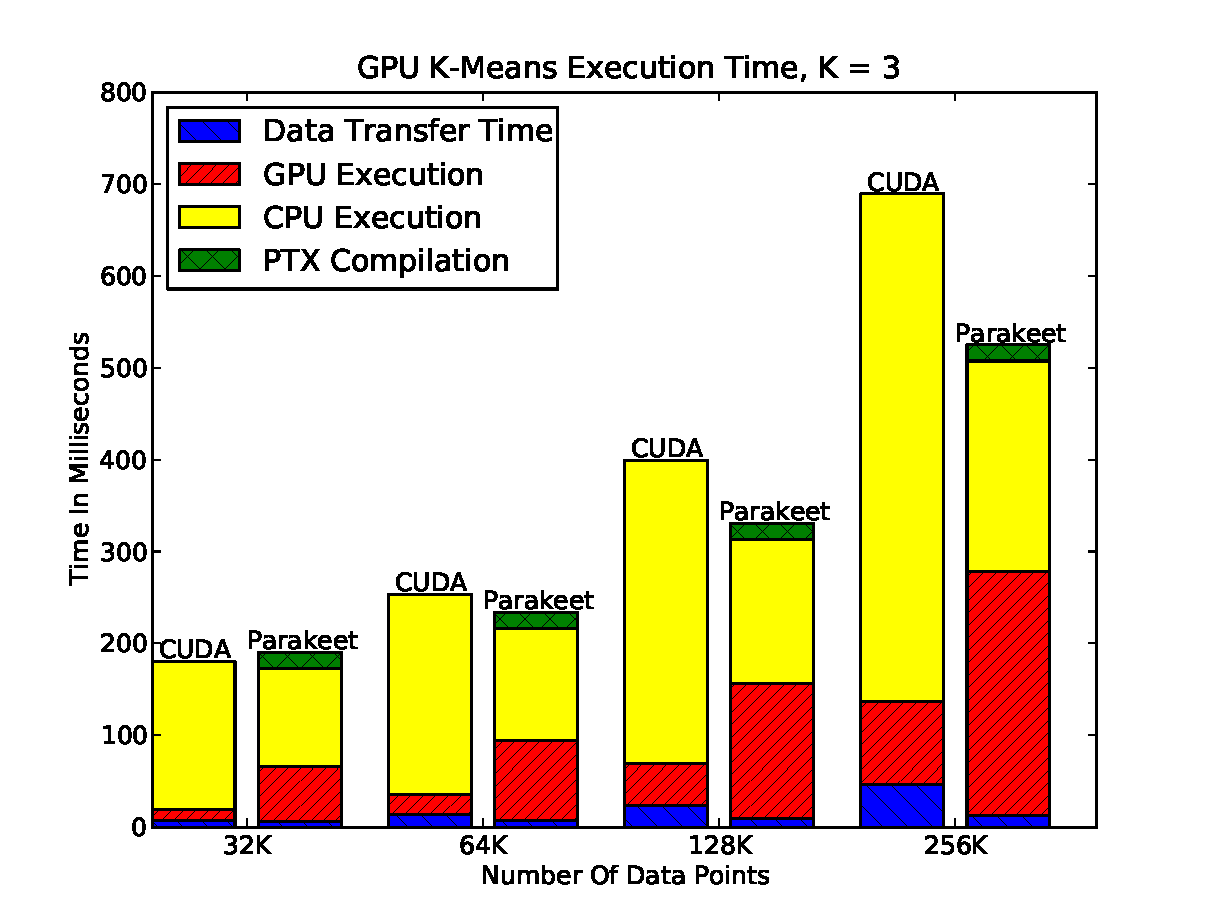
\includegraphics[scale=0.4]{KMGPU.pdf}
\caption{K-Means GPU Times with 30 Features, K = 3}
\label{KMGPU}
\end{figure}

In Figure \ref{KMGPU}, we see a breakdown of the run times for CUDA and Parakeet.  Both Parakeet and the CUDA version use the CPU to perform a significant amount of the computation.  The CUDA version uses the CPU to compute the averages of the new clusters in each iteration, while Parakeet spends a lot of time in its interpreter launching many GPU kernels and performing garbage collection of GPU memory.  In addition, we break down the runtime by reported Parakeet's overhead separately.  This overhead includes initialization costs related to registering functions with the Parakeet runtime; time spent in the Parakeet IL interpreter; and the cost of running the JIT compiler on the generated code.  As can be seen, this overhead is small compared with the overall runtime of the benchmark.

\section{Related Work}
\label{RelatedWork}
There have been several projects that use just-in-time compilation to accelerate Python programs on CPUs, but to our knowledge none have generated parallel code.  The PyPy project is an alternative implementation of Python that includes a JIT compiler and boasts an average 5.3X speedup across 20 benchmarks~\cite{Rigo06}. Psyco was a previous Python JIT compiler that achieved decent speedups~\cite{Rigo04}.  A number of recent projects enable the use of embedded DSLs in Python for various tasks, including SEJITS~\cite{Cook11} and OptiML~\cite{Chaf11}.

The use of graphics hardware for non-graphical computation has a long history~\cite{Leng90}, though convenient frameworks for general purpose GPU programming have only recently emerged. The Brook language extended C with ``kernels'' and ``streams'', exposing a programming model similar to what is now found in CUDA and OpenCL~\cite{Buck04}.  Microsoft's Accelerator~\cite{Tard06} was the first project to use high level (collection-oriented) language constructs as a basis for GPU execution. Accelerator's programming model does not support function abstractions (only expression trees) and its only underlying parallelism construct is limited to the production of $\MAP$-like kernels.  Nikola~\cite{Main10} and Accelerate~\cite{Chak11} are two first-order array-oriented languages embedded within Haskell. Neither is as convenient or feature rich as Parakeet, either requiring the programmer to manually coordinate computations which require multiple GPU kernel launches or lacking support for closures or the nesting of array operators.

Copperhead parallelizes a statically typed, purely functional array subset of Python through the dynamic compilation and execution of CUDA kernels~\cite{Cata11}. Copperhead supports nested array computations, and has a notion of scheduling computation on both GPU and CPU backends (although only a GPU backend has been implemented). In addition to sequentializing nested array operators within CUDA kernels (as done in Parakeet), Copperhead can also share the work of a nested computation among all the threads in a CUDA block. Copperhead does not utilize any dynamic information (such as size) when making these scheduling decisions and thus must rely on user annotations. Copperhead's compiler generates kernels through parameterization of array operator-specific C++ template classes. By using C++ as their backend target, Copperhead has been able to easily integrate the Thrust GPGPU library~\cite{Hobe10} and to offload the bulk of their code optimizations onto a C++ compiler.  However, this results in Copperhead's compile times being the longest of any project mentioned here (orders of magnitude longer than the compiler overhead of Parakeet).

\section{Conclusion}
\label{Conclusion}
Parakeet allows the programmer to write Python code using a widely-used numerical computing library while achieving good performance on modern parallel hardware. Parakeet automatically synthesizes and executes efficient native binaries from Python code. Parakeet is a usable system in which complex programs can be written and executed efficiently.  On two benchmark programs, Parakeet delivers performance very competitive with even hand-tuned GPU implementations.  Parakeet code can coexist with standard Python code, allowing full interoperability with all of Python's tools and libraries.

In the near future, we plan to add support for the generation of multithreaded CPU programs to our CPU backend.  In addition, we plan to increase efficiency by taking advantage of dynamic information, iteratively tuning components of hierarchical algorithms, splitting computation simultaneously across all processors in a system, and doing more to overlap computation with data transfers.

{\small
\bibliographystyle{acm}
\bibliography{../Parallelism}{}
}
\end{document}
